\documentclass{article}
\usepackage[utf8]{inputenc}
\usepackage[T1]{fontenc}
\usepackage[english]{babel}
\setlength{\parindent}{0pt}
\usepackage{hyperref}
\hypersetup{
    colorlinks=true,
    linkcolor=blue,
    filecolor=magenta,      
    urlcolor=cyan}
\usepackage{graphicx}
\graphicspath{ {./pic/} }

\usepackage{fourier,amssymb,microtype,amsmath,gensymb}
\newcommand{\R}{\mathbb{R}}
\usepackage{mdframed,caption,xcolor,enumitem}
\usepackage{tikz,tkz-euclide}

\title{Seminar 2 - Expenditure function}
\author{Xiaoguang Ling \\  \href{xiaoguang.ling@econ.uio.no}{xiaoguang.ling@econ.uio.no}}
\date{\today}

\begin{document}

\maketitle

%%%%%%%%%%%%%%%%%%%%%%%%%%%%%%%%%%%%%%%%%%%%%%%%%%%%%%%%%%%%%%%%%%%%%%%%%%%%%%%%%%%%%%%%%%%%%%
\section{Jehle \& Reny 1.38 - Properties of the Expenditure Function}
Verify that the expenditure function obtained from the CES direct utility function in Example 1.3 
(JR. pp.39) satisfies all the properties given in Theorem 1.7 (JR. pp.37).

\begin{mdframed}[backgroundcolor=blue!20,linecolor=white]

\textbf{Expenditure Function (JR. pp.35)}

\medskip

We define the expenditure function as theminimum-value function:

$$e(p, u) \equiv \min_{x \in \R^n_+} p \cdot x$$

\textbf{Expenditure Function of CES direct utility function (JR. pp.39)}

\medskip

In Example 1.3 (JR. pp.39), we have a so called CES  direct utility function:
$$u(x_1, x_2) = (x_1^{\rho} + x_2^{\rho})^{\frac{1}{\rho}},\ where \ 0 \ne \rho<1.$$

To derive the Expenditure Function, we need to solve the expenditure minimisation problem
given some utility $u$. i.e.
$$\min_{x_1,x_2} \ p_1x_1 + p_2x_2 \ \ s.t.  \ \ u(x_1, x_2) = (x_1^{\rho} + x_2^{\rho})^{\frac{1}{\rho}} = u, \ x_1 \le 0, \ x_2 \le 0$$

(Read JR. pp.40 to see how to minimize the expenditure with Lagrangian method.)

\medskip

The solution to the expenditure-minimisation problem is called the consumer’s
vector of \textbf{Hicksian demands}:

\begin{equation}
    \begin{cases}
    x_1^h(p_1,p_2,u) = u(p_1^{r} + p_2^{r})^{\frac{1}{r}-1} p_1^(r-1) \\	
    x_1^h(p_1,p_2,u) = u(p_1^{r} + p_2^{r})^{\frac{1}{r}-1} p_2^(r-1) \\	
    \end{cases}
    \label{eq:1_38_hicks}   
\end{equation}

Here $r \equiv \frac{\rho}{\rho - 1}$.

Substitute the solution above (Equation \ref{eq:1_38_hicks}) into our
objective function  $p_1x_1 + p_2x_2$ to obtain the Expenditure Function:

$$e(p_1,p_2, u) = p_1x_1^h(p_1,p_2,u) + p_2x_2^h(p_1,p_2,u) = 
u(p_1^{r} + p_2^{r})^{\frac{1}{r}} , r \equiv \frac{\rho}{\rho - 1}$$

\textbf{THEOREM 1.7 Properties of the Expenditure Function (JR. pp.37)}

\medskip

If $u(.)$ is continuous and strictly increasing, then $e(p, u)$ defined in (1.14) is

\begin{enumerate}
\item Zero when $u$ takes on the lowest level of utility in $\mathcal{U}$,
\item Continuous on its domain $\R^n_{++} \times \mathcal{U}$,
\item For all $p \gg 0$, strictly increasing in $u$ and unbounded above in $u$,
\item Increasing in $p$,
\item Homogeneous of degree $1$ in $p$,
\item Concave in $p$.
\end{enumerate}
If, in addition, $u(.)$ is strictly quasiconcave, we have
\begin{enumerate}[start = 7]
\item Shephard’s lemma: $e(p, u)$ is differentiable in $p$ at $(p^0, u^0)$ with $p^0 \gg 0$, and
$$\frac{\partial e(p^0, u^0)}{\partial p_i} = x^h_i (p^0, u^0), \ \ \ \ i = 1, . . . , n.$$
\end{enumerate}
\end{mdframed}

Firstly we should know that the CES direct utility function $u(x_1, x_2) = (x_1^{\rho} + x_2^{\rho})^{\frac{1}{\rho}},\ where \ 0 \ne \rho<1.$ is continuous and strictly increasing (can be proved similarly as below), which is the
prerequisite of Theorem 1.7.

%***************************************************
\subsection{$e(p, u)$ is zero when $u$ takes on the lowest level of utility in $\mathcal{U}$}

As usual, we assume non-negative consumption, i.e. $x \in R^n_+$. Since $u(.)$ is strictly increasing,
$u_{min} = u(0,0) = 0$. 

When $u = 0$, we have $e(p,0) = 0 \times (p_1^{r} + p_2^{r})^{\frac{1}{r}} =0$.

\textit{"no consumption, no cost"}

%***************************************************
\subsection{$e(p, u)$ is continuous on its domain $\R^n_{++} \times \mathcal{U}$,}


\begin{mdframed}[backgroundcolor=blue!20,linecolor=white]
For a ONE dimention function $f(x)$, if the derivative at $x = a$ ($f'(a)$) exists, it's differentiable at $x = a$.

If $f(x)$ is differentiable at $x = a$, it's also continuous at $x = a$.

For a higher dimension function, the existance of all partial/directional derivatives is not
sufficient for its differentiability. Here are examples from Wikipedia: \href{https://en.wikipedia.org/wiki/Differentiable_function}{Differentiability in higher dimensions}
\end{mdframed}

\begin{mdframed}[backgroundcolor=yellow!20,linecolor=white]
Good news for your exam:

\textit{"There is no need to prove continuity (or concavity) of higher dimension functions (in your exam). I might ask you to prove continuity (or concavity) wrt one variable (a specific price, for example)." -- Paolo}
\end{mdframed}

$e(p_1,p_2,u)$ is a 3-dimension function. If you really want to prove it's differentiable/continuous, you can either try to use the definition of differentiable/ continuous functions. 
You can also read theorem A2.21 (Jehle \& Reny pp.602) and theorem 1.9 (point 3,Jehle \& Reny
 pp.520).

For this sub-question, let's assume the prices are given (say, by the market). Therefore
$e(p_1,p_2,u) = e(u)$ is one dimesional.

Obviously, $$\frac{d e(u)}{d u} = \frac{d u(p_1^{r} + p_2^{r})^{\frac{1}{r}} }{d u} = (p_1^{r} + p_2^{r})^{\frac{1}{r}}$$

The derivetive exists for any $u \in \mathcal{U}$. $e(u)$ is differentiable and thus continuous.


%***************************************************
\subsection{For all $p \gg 0$, $e(p, u)$ is strictly increasing in $u$ and unbounded above in $u$,}


Since $\frac{d e(u)}{d u} = (p_1^{r} + p_2^{r})^{\frac{1}{r}} > 0, \forall p \gg 0$,
$e(p_1,p_2,u)$ is strictly increasing in $u$.

Given the positive prices, $\lim_{u\to\infty} e(u) = \lim_{u\to\infty} u(p_1^{r} + p_2^{r})^{\frac{1}{r}}= + \infty$. It there is no upper boundary in $u$.


%***************************************************
\subsection{$e(p, u)$ is increasing in $p$,}

$$\frac{\partial e(p_1,p_2, u)}{\partial p_1} = \frac{\partial u(p_1^{r} + p_2^{r})^{\frac{1}{r}} }{\partial p_1} = u \cdot \frac{1}{r}(p_1^{r} + p_2^{r})^{\frac{1}{r} - 1} \cdot r  p_1^{r-1} =
u (p_1^{r} + p_2^{r})^{\frac{1}{r} - 1} p_1^{r-1} > 0$$

$$\frac{\partial e(p_1,p_2, u)}{\partial p_2} = \frac{\partial u(p_1^{r} + p_2^{r})^{\frac{1}{r}} }{\partial p_2} = u \cdot \frac{1}{r}(p_1^{r} + p_2^{r})^{\frac{1}{r} - 1} \cdot r  p_2^{r-1} =
u (p_1^{r} + p_2^{r})^{\frac{1}{r} - 1} p_2^{r-1} > 0$$

Therefore $e(p, u)$ is increasing in $p$.


%***************************************************
\subsection{$e(p, u)$ is homogeneous of degree $1$ in $p$,}

\begin{mdframed}[backgroundcolor=blue!20,linecolor=white]
Homogeneous functions (Jehle \& Reny Definition A2.2 pp.561):

$f(x)$ is called homogeneous of degree $k$ if $f(tx) \equiv t^kf(x),\ \forall t > 0$

You want to show $e(tp, u) = t^1e(p, u),\ \forall t > 0$
\end{mdframed}

For any $t>0$,

\begin{align*}
e(u,tp) &= u[(tp_1)^{r} + (tp_2)^{r}]^{\frac{1}{r}} \\
&= u[t^r(p_1^{r} + p_2^{r})]^{\frac{1}{r}} \\
&= tu(p_1^{r} + p_2^{r})^{\frac{1}{r}} \\
&= t^1e(u,p)
\end{align*}

Therefore $e(p, u)$ is homogeneous of degree $1$ in $p$.

%***************************************************
\subsection{$e(p, u)$ is concave in $p$.}

\begin{mdframed}[backgroundcolor=blue!20,linecolor=white]
Concave functions (Jehle \& Reny pp.534):

$f : D \to \R \ $ is a concave function if for all $x^1, x^2 \in D$,
$$f(x^t) \ge tf(x^1) + (1 − t)f(x^2), \ \forall t \in [0, 1]$$

Where $x^t \equiv tx^1 + (1-t)x^2, t \in [0,1]$

\vspace{2mm}
{\centering
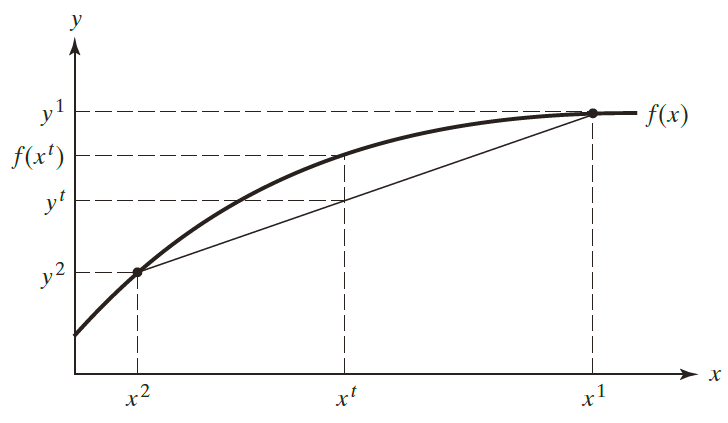
\includegraphics[width=0.8\textwidth]{2.concavef}
\captionof{figure}{Concave functions}
\label{cf}}
\vspace{2mm}

(Diminishing margin)

\begin{itemize}
\item Intuition: $e(p,u)$ is increasing \textbf{in $p$} but the marginal expenditure is diminishing.
\end{itemize}

For this specific function $e(p_1,p_2,u)$, you can follow the very smart proof on Jehle \& Reny pp. 38-39 to show that for any given utility $\bar{u}$, $$e[tp^1+(1-t)p^2,\bar{u}] \ge te(p^1,\bar{u}) + (1-t)e(p^2,\bar{u})$$

Where $p^1 = \left(\begin{smallmatrix}p^1_1 \\ p^1_2\end{smallmatrix}\right)$ and $p^2 = \left(\begin{smallmatrix}p^2_1 \\ p^2_2\end{smallmatrix}\right)$ are two price sets. $t \in [0,1]$

\vspace{2mm}


\textbf{We can also prove it's concavity using derivatives.} 

For a one-dimension increasing function $f(x)$ with diminishing margin (
concave towards x-axis), $f'(x)>0$ and $f''(x)<0$. 

For a higher dimension function $e(p_1,p_2,u)$, it's natural to think about how the derivatives look like.


\vspace{2mm}

We call the second derivatives of a n-demension function $f$ "\textbf{Hessian matrix}" ($H(x)$, Jehle \& Reny pp.557):

\begin{equation}
H(x)=\left(
    \begin{array}{cccc}
		f_{11}(x) & f_{12}(x) & \cdots & f_{1n}(x) \\
		f_{21}(x) & f_{22}(x) & \cdots & f_{2n}(x) \\
		\vdots    &    \vdots & \ddots &   \vdots \\
		f_{n1}(x) & f_{n2}(x) & \cdots & f_{nn}(x) \\
    \end{array}
    \right)
\label{eq:hessian}   
\end{equation}

\vspace{2mm}

We can use the following facts about $H(x)$ and concavity(\href{https://mjo.osborne.economics.utoronto.ca/index.php/tutorial/index/1/qfs/t\#:~:text=Finally\%2C\%20the\%20matrix\%20has\%20one,namely\%20its\%20determinant\%2C\%20\%E2\%88\%9219.&text=A\%20is\%20positive\%20semidefinite\%20if,and\%20nonnegative\%20for\%20k\%20even.}{More details and examples}):

\begin{itemize}
\item  \textbf{Theorem A2.4}(Jehle \& Reny pp.559): If function $f$ is twice continuously differentiable on a convex open set $S$, then 
$f$ is concave $\iff$ the Hessian matrix $H(x)$ of $f$ is \href{https://towardsdatascience.com/what-is-a-positive-definite-matrix-181e24085abd}{negative semidefinite} for all $x \in S$

\item \textbf{Negative semidefinite}(Jehle \& Reny pp.559): a $n \times n$ metrix $H$ is negative semidefinite $\iff \ H$'s $k$th order principal minors are nonpositive for $k$ odd and nonnegative for $k$ even.

\item The $k$th order principal minors of an $n \times n$ symmetric matrix $H$ are the determinants of the $k \times k$ matrices obtained by deleting $n − k$ rows and the corresponding $n − k$ columns of $H$ (where $k = 1, ..., n$).

\end{itemize}

\vspace{2mm}

The Hessian matrix of $e(p_1,p_2,u)$ (in $p$ !) is:

\vspace{2mm}

\begin{equation}
H(p)=\left(
    \begin{array}{cc}
		e_{p_1p_1} & e_{p_1p_2}  \\
		e_{p_2p_1} & e_{p_2p_2}  \\
    \end{array}
    \right) 
\label{eq:hessian_e}   
\end{equation}

\vspace{2mm}

$H(p)$ contains two 1st order ($k = 1, n - k = 2 -1 = 1$) principal minors: $e_{p_1p_1}$ and $e_{p_2p_2}$, and one 2nd order ($k = 2, n - k = 2 -2 = 0$) principal minors:
\begin{equation}
    \begin{vmatrix}
		e_{p_1p_1} & e_{p_1p_2}  \\
		e_{p_2p_1} & e_{p_2p_2}  \\
    \end{vmatrix}
=e_{p_1p_1}e_{p_2p_2} - e_{p_1p_2}e_{p_2p_1}
\label{eq:pminor_e}   
\end{equation}

We want to prove:

\begin{itemize}
\item  $e_{p_1p_1} \le 0$  and $e_{p_2p_2} \le 0$
\item  $e_{p_1p_1}e_{p_2p_2} - e_{p_1p_2}e_{p_2p_1} \ge 0$

\end{itemize}
\end{mdframed}

\vspace{2mm}


We already know $\frac{\partial e(p_1,p_2)}{\partial p_1} =
u (p_1^{r} + p_2^{r})^{\frac{1}{r} - 1} p_1^{r-1}$, and 
$\frac{\partial e(p_1,p_2)}{\partial p_2} = 
u (p_1^{r} + p_2^{r})^{\frac{1}{r} - 1} p_2^{r-1}$


\begin{align*}
\frac{\partial e(p_1,p_2)}{\partial p_1\partial p_1} &=
\frac{\partial u (p_1^{r} + p_2^{r})^{\frac{1}{r} - 1} p_1^{r-1}}{\partial p_1} \\
&= u (\frac{1}{r} - 1)(p_1^{r} + p_2^{r})^{\frac{1}{r} - 2}rp_1^{r-1}p_1^{r-1} + u(p_1^{r} + p_2^{r})^{\frac{1}{r} - 1}(r-1)p_1^{r-2} \\
&= u(p_1^{r} + p_2^{r})^{\frac{1}{r} - 1} p_1^{r-2}[(\frac{1}{r} - 1)(p_1^{r} + p_2^{r})^{-1}rp_1^{r} + (r-1)] \\
&= u(p_1^{r} + p_2^{r})^{\frac{1}{r} - 1} p_1^{r-2} (1-r)[\frac{p_1^{r}}{(p_1^{r} + p_2^{r})} - 1] \\
&= u(p_1^{r} + p_2^{r})^{\frac{1}{r} - 2} p_1^{r-2} (r-1)p_2^r \\
\end{align*}

\begin{equation}
\because \ \ \
    \begin{cases}
u(p_1^{r} + p_2^{r})^{\frac{1}{r} - 2} p_1^{r-2}p_2^r \ge 0 \\
r \equiv \frac{\rho}{\rho - 1} = \frac{1}{1 - \frac{1}{\rho}} < 1, \forall \rho < 1, \rho \ne 0 \Rightarrow r-1 \le 0 \\
    \end{cases}
\nonumber
\end{equation}

$\therefore e_{p_1p_1} \le 0$

Similarly, $e_{p_2p_2} = u(p_1^{r} + p_2^{r})^{\frac{1}{r} - 2} p_2^{r-2} (r-1)p_1^r \le 0$ (note $p_1$ and $p_2$ are "symmetric").

\begin{align*}
\frac{\partial e(p_1,p_2)}{\partial p_1\partial p_2} &=
\frac{\partial u (p_1^{r} + p_2^{r})^{\frac{1}{r} - 1} p_1^{r-1}}{\partial p_2} \\
&= u ({\frac{1}{r} - 1})(p_1^{r} + p_2^{r})^{\frac{1}{r} - 2} rp_2^{r-1}p_1^{r-1} \\
&= u (1-r)(p_1^{r} + p_2^{r})^{\frac{1}{r} - 2} p_2^{r-1}p_1^{r-1} \\
\end{align*}

According to Young's theorem (Jehle \& Reny pp.557),$\frac{\partial e(p_1,p_2)}{\partial p_1\partial p_2} = \frac{\partial e(p_1,p_2)}{\partial p_2\partial p_1}$ 

We have
\begin{align*}
 e_{p_1p_1}e_{p_2p_2} - e_{p_1p_2}e_{p_2p_1} &=
[u(p_1^{r} + p_2^{r})^{\frac{1}{r} - 2} p_1^{r-2} (r-1)p_2^r][u(p_1^{r} + p_2^{r})^{\frac{1}{r} - 2} p_2^{r-2} (r-1)p_1^r] \\ 
& - [u (1-r)(p_1^{r} + p_2^{r})^{\frac{1}{r} - 2} p_2^{r-1}p_1^{r-1}]^2 \\ &=u^2(p_1^{r} + p_2^{r})^{\frac{2}{r} - 4}(p_1p_2)^{2r-2)} (r-1)^2 -
u^2(1-r)^2(p_1^{r} + p_2^{r})^{\frac{2}{r} - 4} (p_2p_1)^{2r-2} \\
&= 0 \ge 0
\end{align*}

Therefore, $H(p)$ is negative semidefinite $\Rightarrow \ e(p,u)$ is concave in $p$.


%***************************************************
\subsection{If $u(.)$ is also strictly quasiconcave, we have Shephard’s lemma: $e(p, u)$ is differentiable in $p$ at $(p^0, u^0)$ with $p^0 \gg 0$, and $\frac{\partial e(p^0, u^0)}{\partial p_i} = x^h_i (p^0, u^0), \ \ \ \ i = 1, . . . , n$.}















%%%%%%%%%%%%%%%%%%%%%%%%%%%%%%%%%%%%%%%%%%%%%%%%%%%%%%%%%%%%%%%%%%%%%%%%%%%%%%%%%%%%%%%%%%%%%%
\section{Jehle \& Reny 1.44 - Inferior and Normal goods}
In a two-good case, show that if one good is inferior, the other good must be normal.




%%%%%%%%%%%%%%%%%%%%%%%%%%%%%%%%%%%%%%%%%%%%%%%%%%%%%%%%%%%%%%%%%%%%%%%%%%%%%%%%%%%%%%%%%%%%%%
\section{Jehle \& Reny 1.51 - Substitues and Complements}
Consider the utility function, $u(x_1, x_2) = (x_1)^{1/2} + (x_2)^{1/2}$.

\begin{enumerate}[label=\alph*.]

\item Compute the demand functions, $x_i(p_1, p_2, y), \ i = 1, 2$.

\item Compute the substitution term in the Slutsky equation for the effects on $x_1$ of changes in $p_2$.

\item Classify $x_1$ and $x_2$ as (gross) complements or substitutes.

\end{enumerate}



\begin{figure}

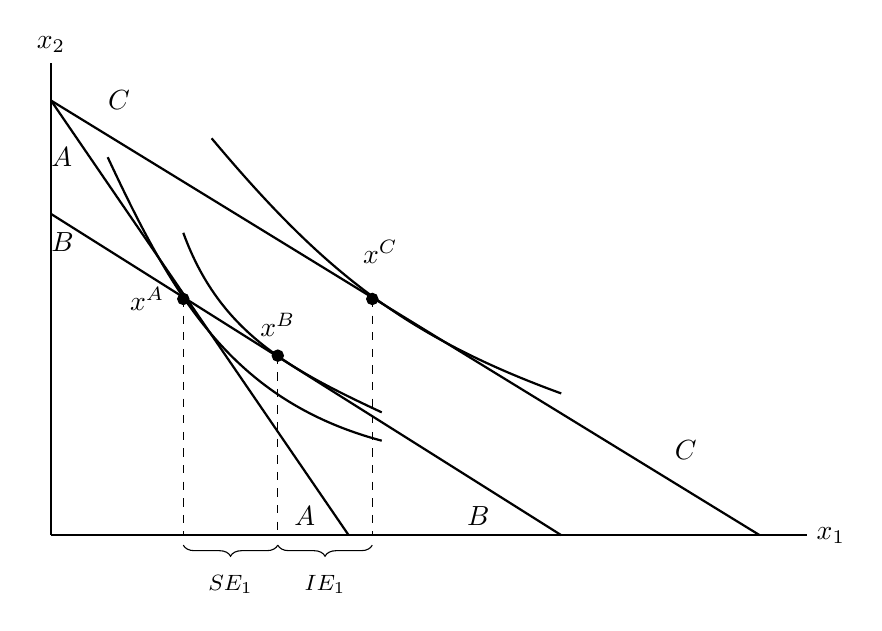
\begin{tikzpicture}[scale=1.2]

\draw [thick] (0,0) -- (8,0);
\draw [thick] (0,0) -- (0,5);
\node [right] at (8,0) {$x_1$};
\node [above] at (0,5) {$x_2$};
\draw [thick] (1.7,4.2) to [out=310,in=160] (5.4,1.5);
\draw [thick] (0.6,4) to [out=295,in=165] (3.5,1);
\draw [thick] (1.4,3.2) to [out=290,in=155] (3.5,1.3);
\node [right] at (6.5,0.9) {$C$};
\draw [thick] (0,4.6) -- (7.5,0);
\draw [thick] (0,4.6) -- (3.15,0);
\draw[dashed](1.4,2.5)--(1.4,0);
\draw[dashed](3.4,2.5)--(3.4,0);
\draw [thick] (0,3.4) -- (5.4,0);
\draw[dashed](2.4,1.9)--(2.4,0);
\node [above] at (2.4,2) {$x^B$};
\draw[fill] (2.4,1.9) circle [radius =0.06];
\node [left] at (1.3,2.5) {$x^A$};
\draw[fill] (1.4,2.5) circle [radius =0.06];
\node [right] at (3.2,3) {$x^C$};
\draw[fill] (3.4,2.5) circle [radius =0.06];
\node [right] at (0.5,4.6) {$C$};
\node [right] at (-0.1,4) {$A$};
\node [left] at (2.9,0.2) {$A$};
\node [right] at (4.3,0.2) {$B$};
\node [right] at (-0.1,3.1) {$B$};
\draw [decorate,decoration={brace,amplitude=4pt, mirror},xshift=0pt,yshift=-3pt]
(1.4,0) -- (2.4,0) node [black,midway,yshift=-.5cm] {\footnotesize $SE_1$};
\draw [decorate,decoration={brace,amplitude=4pt, mirror},xshift=0pt,yshift=-3pt]
(2.4,0) -- (3.4,0) node [black,midway,yshift=-.5cm] {\footnotesize $IE_1$};
\end{tikzpicture}
\caption{Slutsky decomposition}
\end{figure}
\end{document}